\chapter{Design considerations for a heterodyne interferometer}
\label{ch:DesignConsiderations}
While Chapter~\ref{ch:InterferometricMethods} discusses the
\emph{optical} foundations for various interferometric methods,
most real-world optical diagnostics are complex, integrated systems
requiring precise interplay between various components, such as
lasers, optics, detectors, and electronics.
Optimizing the performance of a given diagnostic
requires careful consideration
of each component and its role in the measurement.
Some of these considerations are generic, and
some of them are diagnostic specific.

This chapter examines numerous design considerations
that are relevant to heterodyne interferometry.
The sections are arranged in roughly sequential order,
beginning with the interference signal at the detector and
proceeding through successive downstream components
until reaching the system's digitizer.
In particular, Section~\ref{sec:DesignConsiderations:geometric}
discusses the geometric effects that
affect the magnitude of the heterodyne signal and
set the wavenumber response of the interferometer.
Section~\ref{sec:DesignConsiderations:intensity}
explores heterodyne measurements made
beyond the saturation-intensity limit of a given detector.
Sections~\ref{sec:DesignConsiderations:phase_noise} and
\ref{sec:DesignConsiderations:amplitude_noise}
reveal how phase noise and amplitude noise, respectively,
can creep into the interferometer's measurements.
Section~\ref{sec:DesignConsiderations:demodulation}
describes demodulation of the heterodyne interference signal and
the distortion of the baseband phase signal
that results from demodulator imperfections.
Finally, Section~\ref{sec:DesignConsiderations:quantization}
discusses the signal quantization
that necessarily occurs
when generating a digital record.
The below design considerations will be referenced extensively in
Chapter~\ref{ch:Implementation}, which
describes the addition of a heterodyne interferometer
to the pre-existing phase contrast imaging (PCI) diagnostic
on the \diiid\space tokamak.


\section{Geometric considerations}
\label{sec:DesignConsiderations:geometric}
Several geometric effects substantially influence
the performance of a heterodyne interferometer.
Section~\ref{sec:DesignConsiderations:geometric:aperture_diffraction}
provides a minimum threshold on the radii of components in the optical train,
while Section~\ref{sec:DesignConsiderations:geometric:beam_coalignment}
derives the required degree of coalignment between
the probe beam and the reference beam.
Section~\ref{sec:DesignConsiderations:geometric:beam_mismatch}
discusses the implications of mismatches between
the spatial structures of the probe beam and the reference beam and
develops a criterion for the required level of matching.
Section~\ref{sec:DesignConsiderations:geometric:finite_sampling_volume}
reveals how the imaging system's magnification $M$ and
the detector's size and shape
influence the interferometer's wavenumber response.


\subsection{Aperture diffraction}
\label{sec:DesignConsiderations:geometric:aperture_diffraction}
Diffraction from finite-aperture optics was neglected in
Chapter~\ref{ch:InterferometricMethods}'s
transfer-function derivations.
For a propagating Gaussian beam,
this neglect of aperture diffraction is a reasonable approximation if
\begin{equation}
  a_{\text{eff}} \geq \frac{3}{2} w(z),
  \label{eq:DesignConsiderations:aperture_radius_for_minimal_diffraction}
\end{equation}
for each aperture, where
$a_{\text{eff}}$ is the effective aperture radius and
$w(z)$ is the beam's 1/e $E$ radius at the aperture location
\cite{campbell_josa69, rost_diffraction_pc14}.
For a circular aperture of radius $a$,
the effective aperture radius is simply $a_{\text{eff}} = a$
for a beam propagating along the optical axis
(e.g.\ the unscattered beam from
Sec.~\ref{sec:InterferometricMethods:Gaussian_beam_diffraction:from_plasma_density_fluctuations});
however, for a beam located $\rho(z)$ away from the optical axis
(e.g.\ the upscattered or downscattered beam from
Sec.~\ref{sec:InterferometricMethods:Gaussian_beam_diffraction:from_plasma_density_fluctuations}),
the effective aperture radius is $a_{\text{eff}} = a - |\rho(z)|$.


\subsection{Beam coalignment}
\label{sec:DesignConsiderations:geometric:beam_coalignment}
For the moment, assume a plane-wave representation
for both the reference beam and the unscattered probe beam.
Specifically, let the reference beam be given by
\begin{equation}
  \vect{E}_R(\vect{r})
  =
  E_0 \hat{\vect{x}}
  \cdot
  e^{i [k_0 z - (\omega_0 + \Delta \omega_0)t]},
\end{equation}
and let the unscattered probe beam
be misaligned with the reference beam
by angle $\theta \ll 1$ such that,
to lowest order in $\theta$,
the unscattered probe beam is
\begin{equation}
  \vect{E}_P(\vect{r})
  \approx
  E_0 \hat{\vect{x}}
  \cdot
  e^{i [k_0 (z + \theta x) - \omega_0 t]}.
\end{equation}
The total intensity (averaged over an optical cycle) is then
\begin{align}
  I
  =
  \frac{c \varepsilon_0}{2}
  \left|
    \vect{E}_R + \vect{E}_P
  \right|^2
  \approx
  2 I_0 \left[ 1 + \cos(\Delta \omega_0 t + k_0 \theta x) \right],
\end{align}
where $I_0 = c \varepsilon_0 E_0^2 / 2$
is the corresponding intensity of a single beam.
Here, the cosine term
corresponds to the interference between the two beams, and
the unity term corresponds to the intensity of each individual beam.
Optimizing the interference signal requires
alignment of the beam polarizations and
minimization of the misalignment angle $\theta$.
If the interference is measured by a detector
with an extent $s_x$ in the $x$-direction,
the misalignment-induced phase $k_0 \theta x$
should change by much less than $2 \pi$ across the detector face;
i.e.\ $|k_0 \theta s_x| \ll 2 \pi$ or
\begin{equation}
  |\theta|
  \ll
  \frac{\lambda_0}{s_x}
  \approx
  0.6^{\circ},
  \label{eq:DesignConsiderations:coalignment_constraint}
\end{equation}
where $\lambda_0 = 2 \pi / k_0$ is the beam wavelength, and
$\lambda_0 = \SI{10.6}{\micro\meter}$ and
$s_x = \SI{1}{\milli\meter}$
have been used for the evaluation.
Coalignment constraint (\ref{eq:DesignConsiderations:coalignment_constraint})
has design implications for CO$_2$ interferometers
that are built for magnetic fusion experiments, which
are often characterized by large, pulsed electromagnets
whose operation may contort the machine and produce vibrations,
potentially destroying the beam coalignment.


\subsection{Mismatch between beam spatial structures}
\label{sec:DesignConsiderations:geometric:beam_mismatch}
The external reference-beam interferometry derivations
in Section~\ref{sec:InterferometricMethods:interferometry}
assumed that the reference beam was exactly matched
in both amplitude and spatial structure
to the unscattered probe beam.
This is obviously an idealization
that, at best, can only be approximately met in experiment.
This section discusses the geometric effects
of such imperfections in beam matching.

The derivation of the heterodyne intensity
(\ref{eq:InterferometricMethods:heterodyne_intensity})
can be easily generalized to account for
the geometric effects of unmatched reference and probe beams.
Namely, let the image-plane probe radiation be given by
(\ref{eq:InterferometricMethods:imaged_total_field_interferometer}) as
\begin{equation}
  E_P(\vect{r}_{\image}, t)
  \approx
  E_{G,P}(\vect{r}_{\image}, t)
  e^{i \bar{\phi}}
  \left[%
    1
    +
    i \tilde{\phi}(x_{\image}, t)
  \right],
\end{equation}
and let the corresponding reference beam be given by
\begin{equation}
  E_R(\vect{r}_{R}, t)
  =
  E_{G,R}(\vect{r}_{R}, t) e^{-i \Delta\omega_0 t},
\end{equation}
where $\vect{r}_{\image} = (x_{\image}, y_{\image}, z_{\image})$,
\begin{equation}
  \vect{r}_{R}
  =
  \vect{r}_{\image}
  +
  (0, 0, z_{R} - z_{\image}),
\end{equation}
and $E_{G,j}$ is a Gaussian beam
with angular frequency $\omega_0$,
waist amplitude $E_{0,j}$, and
waist 1/e $E$ radius $w_{0,j}$.
If $z_R \neq z_{\image}$,
the reference beam's waist sits at a different location
than that of the unscattered probe beam.
Under these circumstances, the heterodyne intensity becomes
\begin{equation}
  \begin{aligned}
    I_{\text{het}}(\vect{r}_{\image}, z_R, t)
    =
    2 I_{G,P}(\vect{r}_{\image})
    \bigl[%
      &\alpha_{\text{DC}}
      +
      \alpha_{\text{AC}}
      \cos(\Delta \omega_0 t + \bar{\phi}_{\text{eff}})
      \\
      &-
      \alpha_{\text{AC}}
      \tilde{\phi}(x_{\image}, t)
      \sin(\Delta \omega_0 t + \bar{\phi}_{\text{eff}})
    \bigr],
  \end{aligned}
  \label{eq:DesignConsiderations:heterodyne_intensity}
\end{equation}
where
\begin{equation}
  \bar{\phi}_{\text{eff}}
  =
  \bar{\phi}
  +
  \bigl[ \phi_{G,P}(\vect{r}_{\image}) - \phi_{G,R}(\vect{r}_R) \bigr]
\end{equation}
is the effective bulk phase,
\begin{equation}
  \phi_{G,j}(\vect{r})
  =
  k_0 z + \frac{k_0 \rho^2}{2 R_j(z)} - \psi_j(z)
\end{equation}
is the phase of Gaussian beam $j \in \{P, R\}$
(i.e.\ $E_{G,j}(\vect{r}) = |E_{G,j}(\vect{r})| e^{i \phi_{G,j}(\vect{r})}$),
\begin{align}
  \alpha_{\text{DC}}
  &=
  \frac{1 + \alpha_{\text{AC}}^2}{2},
  \\
  \alpha_{\text{AC}}
  &=
  \sqrt{\frac{I_{G,R}(\vect{r}_R)}{I_{G,P}(\vect{r}_{\image})}},
\end{align}
are geometric factors that describe the amplitudes
of the DC and AC components of the heterodyne signal, and
\begin{equation}
  I_{G,j}(\vect{r})
  =
  \frac{c \varepsilon_0 |E_{G,j}(\vect{r})|^2}{2}
\end{equation}
is the intensity profile (averaged over an optical cycle)
of Gaussian beam $j \in \{P, R\}$.
Note that (\ref{eq:DesignConsiderations:heterodyne_intensity})
readily reduces to (\ref{eq:InterferometricMethods:heterodyne_intensity})
if $E_{G,R}(\vect{r}_R) = E_{G,P}(\vect{r}_{\image})$.

It is worth discussing the implications of heterodyne intensity
(\ref{eq:DesignConsiderations:heterodyne_intensity}).
First, repeating the derivation between
(\ref{eq:InterferometricMethods:heterodyne_interferometer_I_and_Q_intensity})
and
(\ref{eq:InterferometricMethods:heterodyne_interferometer_wavenumber_transfer_function})
with this modified heterodyne intensity,
one readily finds that
the heterodyne interferometer's wavenumber transfer function
(\ref{eq:InterferometricMethods:heterodyne_interferometer_wavenumber_transfer_function})
should be multiplied by the factor
$2 \alpha_{\text{AC}} / (\alpha_{\text{DC}} + \alpha_{\text{AC}})$.
It is then easy to show that
the transfer function is \emph{maximized} when
$\alpha_{\text{DC}} = \alpha_{\text{AC}} = 1$,
i.e.\ when the probe beam and reference beam
have identical spatial structures and powers.
Second, note that the effective bulk phase $\bar{\phi}_{\text{eff}}$
is dependent on the geometry of the reference beam and
the unscattered probe beam.
Specifically, in the context of measuring
the plasma-induced bulk phase $\bar{\phi}$,
note that
\begin{equation}
  \bar{\phi}_{\text{eff}}(\rho_{\image}=0)
  =
  \bar{\phi}
  +
  k_0 (z_{\image} - z_R)
  -
  \left[ \psi_P(z_{\image}) - \psi_R(z_R) \right].
\end{equation}
If $z_{\image}$ and $z_R$ are fixed,
then the beam-geometry contributions to
$\bar{\phi}_{\text{eff}}(\rho_{\image} = 0)$
constitute an unimportant DC offset that can be removed
via baseline subtraction;
however, experiments are typically plagued by vibrations, and
even small changes to $z_{\image}$ and $z_R$
can make significant time-dependent contributions to
$\bar{\phi}_{\text{eff}}(\rho_{\image} = 0)$ at CO$_2$ probe wavelengths.
As such, deconvolving the plasma-induced and vibration-induced contributions
to $\bar{\phi}_{\text{eff}}(\rho_{\image} = 0)$
requires interferometric measurements
at two distinct wavelengths (i.e.\ two-color interferometry)
\cite{carlstrom_rsi88}.
However, such vibrations occur on slow time-scales
(e.g.\ $f_{\text{vib}} \lesssim \SI{5}{\kilo \hertz}$),
and phase measurements at a \emph{single} wavelength are sufficient
to quantify plasma-induced phase fluctuations
at frequencies above $f_{\text{vib}}$
\cite{vanzeeland_ppcf05}.
Finally, note that the beam geometry also imparts
a spatially dependent, curvature-induced phase shift
\begin{align}
  \delta\phi_{\kappa}(\rho_{\image})
  &=
  \bar{\phi}_{\text{eff}}(\rho_{\image})
  -
  \bar{\phi}_{\text{eff}}(\rho_{\image} = 0)
  \notag \\
  &=
  \frac{k_0 \rho_{\image}^2}{2}
  \left[\frac{1}{R_P(z_{\image})} - \frac{1}{R_R(z_R)} \right],
\end{align}
which can result in signal loss and distortion of the measured wavenumber.
To see this, assume that the radiation is interfered on a detector array,
as shown in Fig.~\ref{fig:DesignConsiderations:detector_array}.
As a detector element produces a signal
proportional to the average intensity across its face,
there will be substantial signal loss
if there are large curvature-induced phase shifts
across the element's face
(i.e.\ $\delta\phi_{\kappa}(s_x / 2) \gtrsim \pi$ or
$\delta\phi_{\kappa}(s_y / 2) \gtrsim \pi$).
Further, if there are large curvature-induced phase shifts
across the length of the detector array,
the spatial structure of the intensity
will \emph{not} correspond to the spatial structure
of the plasma fluctuation.
The latter is the more conservative constraint
on the curvature-induced phase shift.
Assuming that the detector array shown in
Fig.~\ref{fig:DesignConsiderations:detector_array}
consists of $N_{\text{el}}$ detector elements and
that the inter-element spacing is negligible ($\delta_x \ll s_x$),
the criterion for negligible curvature-induced phase shifts
$\delta\phi_{\kappa, \text{max}}
=
\delta\phi_{\kappa}(\rho_{\image, \text{max}})
\ll
\pi$
becomes
\begin{equation}
  \frac{k_0}{8}
  \left[ (N_{\text{el}} s_x)^2 + s_y^2 \right]
  \left| \frac{1}{R_P(z_{\image})} - \frac{1}{R_R(z_R)}\right|
  \ll
  \pi.
\end{equation}

\begin{figure}
  \centering
  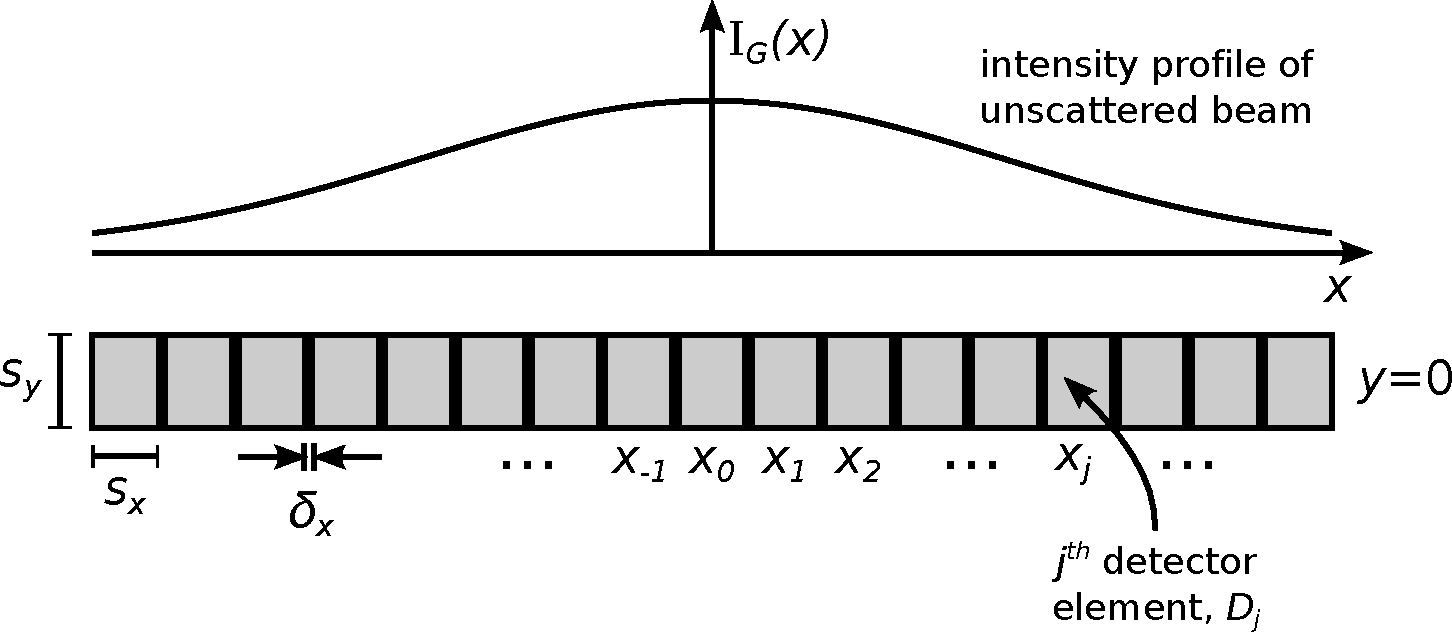
\includegraphics[width = \textwidth]{%
    Chapters/DesignConsiderations/figs/detector_array.pdf}
  \caption[Finite sampling volumes in a detector array]{%
    The probe radiation and the reference beam
    are interfered on a detector array.
    The array consists of numerous detector elements,
    each of size $s_x \times s_y$ and with interelement spacing $\delta_x$.
    The unscattered beam is centered on $x = x_0$ and $y = 0$, and
    its intensity profile varies only weakly over any given element.
    The finite size of each detector element tends to attenuate
    short wavelength components of the incident optical signal.
  }
\label{fig:DesignConsiderations:detector_array}
\end{figure}


\subsection{Finite sampling-volume effects}
\label{sec:DesignConsiderations:geometric:finite_sampling_volume}
Practically speaking, detection is always effected
via detector elements of \emph{finite} size,
with the output of each detector element
corresponding to the incident intensity
\emph{averaged} over the element's active area.
This averaging acts as a low-pass filter in the spatial domain and
is referred to as the finite sampling-volume effect~\cite{bravenec_rsi95}.

Finite sampling-volume effects dictate
a heterodyne interferometer's wavenumber response~\cite{davis_rsi16}.
To see this, assume that measurements
are made with the detector array shown in
Fig.~\ref{fig:DesignConsiderations:detector_array}.
Let the $j$\ts{th} detector element $D_j$ be centered on $x_{\image,j}$
and $y_{\image} = 0$.
Integrating the optical intensity $\tilde{I}_{IQ}(\vect{r}_{\image}, t)$
corresponding to fluctuations in the baseband signal from
(\ref{eq:InterferometricMethods:heterodyne_total_fluctuating_intensity})
over the face of detector element $D_j$ yields
the corresponding optical power
\begin{align}
  \tilde{P}_{IQ,j}(t)
  &=
  \int_{D_j} \tilde{I}_{IQ}(\vect{r}_{\image}, t) dA
  \notag \\
  &\approx
  \frac{2 \sqrt{2}}{\pi}
  I_G(\vect{r}_{\image,j}) s_y
  \int_{x_{\image,j} - s_x / 2}^{x_{\image,j} + s_x / 2}
  \tilde{\phi}(x_{\image}, t)
  dx_{\image};
  \label{eq:DesignConsiderations:fluctuating_baseband_equivalent_optical_power_per_element_v1}
\end{align}
here, the intensity profile $I_G(\vect{r}_{\image})$
has been assumed to be approximately constant
over the face of the detector element.
Because (\ref{eq:DesignConsiderations:fluctuating_baseband_equivalent_optical_power_per_element_v1})
is linear in $\tilde{\phi}$,
it is suitable to consider a single Fourier mode
\begin{equation}
  \tilde{\phi}(x_{\image}, t)
  =
  \tilde{\phi}_0 \cos(k_{\image} x_{\image} - \omega t)
\end{equation}
for which (\ref{eq:DesignConsiderations:fluctuating_baseband_equivalent_optical_power_per_element_v1})
reduces to
\begin{equation}
  \tilde{P}_{IQ,j}(t)
  =
  \frac{2 \sqrt{2}}{\pi}
  I_G(\vect{r}_{\image,j}) A
  \cdot
  T_{\text{fsv}}(k_{\image})
  \cdot
  \tilde{\phi}_0 \cos(k_{\image} x_{\image} - \omega t),
  \label{eq:DesignConsiderations:fluctuating_baseband_equivalent_optical_power_per_element_v2}
\end{equation}
where $A = s_x s_y$ is the area of the detector element,
\begin{equation}
  T_{\text{fsv}}(k_{\image})
  \equiv
  \sinc\left( \frac{k_{\image}}{k_{\text{fsv},\image}} \right)
  \label{eq:DesignConsiderations:finite_sampling_volume_transfer_function}
\end{equation}
is the finite sampling-volume transfer function,
\begin{equation}
  \sinc(x) = \frac{\sin(\pi x)}{\pi x}
  \label{eq:DesignConsiderations:normalized_sinc}
\end{equation}
is the normalized sinc function, and
\begin{equation}
  k_{\text{fsv},\image} = \frac{2 \pi}{s_x}
  \label{eq:DesignConsiderations:finite_sampling_volume_cutoff_image_plane}
\end{equation}
is the first zero of $T_{\text{fsv}}(k_{\image})$.
Recalling that an object-plane wavenumber $k$
is imaged as $k_{\image} = k / M$
in a magnification-$M$ imaging system,
the corresponding object-plane finite sampling-volume wavenumber cutoff is
\begin{equation}
  k_{\text{fsv}} = \frac{2 \pi M}{s_x}.
  \label{eq:DesignConsiderations:finite_sampling_volume_cutoff}
\end{equation}
Now, as in Section~\ref{sec:InterferometricMethods:interferometry:heterodyne},
select the central intensity of the unscattered beam at the detector to be
$I_G(0) = I_{\text{sat}} / 4$, where
$I_{\text{sat}}$ is the detector's linear saturation intensity,
such that
\begin{equation}
  \frac{\tilde{P}_{IQ,j}(t)}{I_{\text{sat}} A}
  =
  \frac{I_G(\vect{r}_{\image,j})}{I_G(0)}
  \cdot
  T_{\text{het}}(k_{\image})
  \cdot
  \tilde{\phi}_0 \cos(k_{\image} x_{\image} - \omega t),
\end{equation}
where
\begin{equation}
  T_{\text{het}}(k_{\image})
  =
  \frac{1}{\sqrt{2} \cdot \pi} \cdot T_{\text{fsv}}(k_{\image})
  \label{eq:DesignConsiderations:heterodyne_interferometer_wavenumber_transfer_function}
\end{equation}
is the heterodyne interferometer's wavenumber transfer function.
In the limit $s_x \rightarrow 0$, $T_\text{fsv} \rightarrow 1$ and
the heterodyne interferometer's wavenumber transfer function reduces to
(\ref{eq:InterferometricMethods:heterodyne_interferometer_wavenumber_transfer_function}).
Thus, finite sampling-volume effects
introduce a wavenumber dependence into $T_{\text{het}}$,
as shown in Fig.~\ref{fig:DesignConsiderations:fsv_effects}.
Note that finite sampling-volume effects
introduce similar wavenumber dependencies
into the transfer functions of the homodyne interferometer and PCI.

\begin{figure}
  \centering
  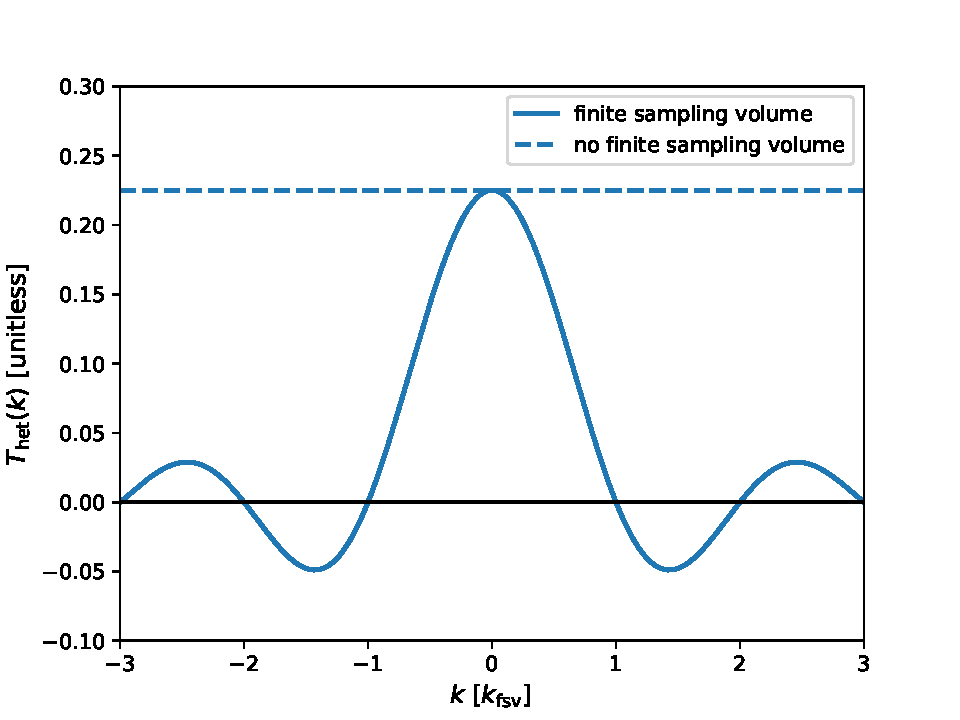
\includegraphics[width = \textwidth]{%
    Chapters/DesignConsiderations/figs/fsv_effects.pdf}
  \caption[Transfer function of heterodyne interferometer with finite sampling-volume effects]{%
    The wavenumber transfer function for a heterodyne interferometer
    with finite sampling-volume effects and
    without finite sampling-volume effects.
  }
\label{fig:DesignConsiderations:fsv_effects}
\end{figure}


\section{Intensity considerations}
\label{sec:DesignConsiderations:intensity}
Ideally, a photovoltaic detector produces an output voltage
\begin{equation}
  V(t) = \mathcal{R}_0 \cdot I(t),
\end{equation}
where $\mathcal{R}_0$ is the detector responsivity and
$I(t)$ is the incident optical intensity.
However, every real-world detector has a saturation intensity $I_{\text{sat}}$
beyond which the output voltage ceases to be a linear function
of the incident optical intensity; that is,
the detector responsivity has an intensity dependence $\mathcal{R}(I)$, and
the detector voltage can be more generally written as
\begin{equation}
  V(t) = \mathcal{R}\left( I(t) \right) \cdot I(t).
\end{equation}
Here, $\mathcal{R}(I)$ is an arbitrary monotonically increasing function
of the incident optical intensity $I$.
Despite the potentially nonlinear response,
the detector voltage remains periodic in $2 \pi / \Delta \omega_0$ and
can be expanded in a Fourier series as
\begin{equation}
  V(t)
  =
  V_0
  +
  \sum_{n = 1}^{\infty}
  V_n \cos\left( n \Delta \omega_0 t + \theta_n \right),
\end{equation}
where $V_n$ and $\theta_n$ are the amplitude and phase, respectively,
of the $n\ts{th}$ harmonic.
Thus, a nonlinear detector response produces
higher-order harmonics in the signal.
In general, $V_n$ and $\theta_n$ can vary in time,
producing sidebands about each harmonic.
Provided the bandwidth of these fluctuations is sufficiently low,
there will be no spectral overlap
between the sidebands of adjacent harmonics, and
bandpass filtering the detector signal about $\Delta \omega_0$ yields
\begin{equation}
  V(t) \approx V_1 \cos[\Delta \omega_0 t + \theta_1(t)]
\end{equation}
with $\theta_1(t) = \phi(t)$, where
$\phi(t)$ is the optical phase shift
between the plasma and reference arms of the interferometer.
However, for fluctuations with sufficiently high bandwidth
(e.g.\ $\omega \sim \Delta\omega_0 / 2$),
the sidebands of adjacent harmonics begin to overlap,
potentially corrupting the phase measurement,
as demonstrated by the example in
Fig.~\ref{fig:DesignConsiderations:nonlinear_heterodyne_detection}.
When operating in the saturated regime,
the heterodyne interferometer's wavenumber transfer function
(\ref{eq:DesignConsiderations:heterodyne_interferometer_wavenumber_transfer_function})
should be multiplied by the prefactor $(V_1 / V_{\text{sat}})$, where
$V_1$ is the amplitude of the heterodyne frequency's fundamental harmonic and
$V_{\text{sat}}$ is the output voltage of the detector
when the incident optical intensity
is equal to the saturation intensity $I_{\text{sat}}$.

\begin{figure}
  \centering
  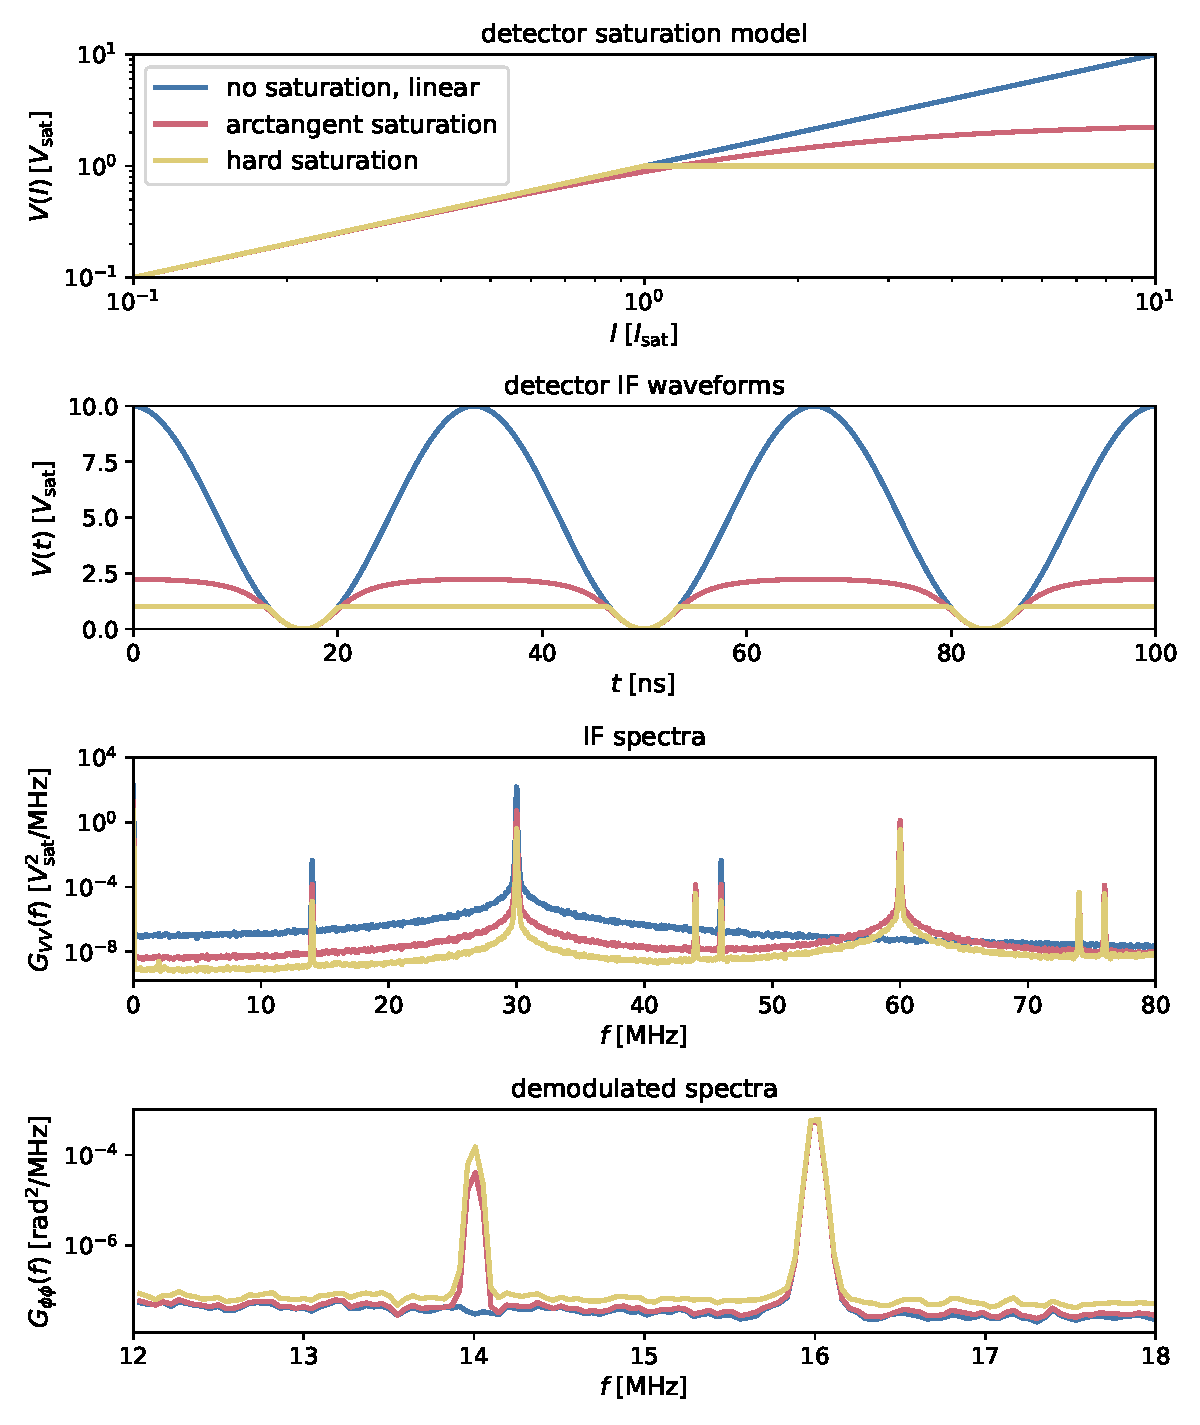
\includegraphics[width = \textwidth]{%
    Chapters/DesignConsiderations/figs/nonlinear_heterodyne_detection.pdf}
  \caption[Heterodyne detection beyond the saturation intensity]{%
    Heterodyne detection beyond the saturation intensity with
    $\Delta\omega_0 = 2\pi \cdot \SI{30}{\mega\hertz}$ and
    $\omega = 2 \pi \cdot \SI{16}{\mega\hertz}$.
    (Top panel): Various detector saturation models.
    The linear model exhibits no saturation,
    the hard saturation model limits the output voltage
    to $V_{\text{sat}}$ when the incident optical intensity
    exceeds $I_{\text{sat}}$, and
    the arctangent saturation model exhibits $\SI{1}{\deci\bel}$ compression
    when the incident optical intensity is $I_{\text{sat}}$.
    (2\ts{nd} panel): The intermediate frequency (IF) waveforms
    corresponding to each saturation model when
    $I_{\text{max}} = 10 \, I_{\text{sat}}$.
    The arctangent and hard saturation models distort the IF waveform,
    producing numerous higher-order harmonics.
    (3\ts{rd} panel): Autospectral densities of the IF waveforms.
    The IF waveforms all exhibit peaks at
    the $\SI{30}{\mega\hertz}$ fundamental and
    its corresponding sidebands at
    $\SI{30}{\mega\hertz} \pm \SI{16}{\mega\hertz}$.
    However, the saturated IF waveforms
    also exhibit peaks at the second harmonic ($\SI{60}{\mega\hertz}$)
    and its corresponding sidebands
    ($\SI{60}{\mega\hertz} \pm \SI{16}{\mega\hertz}$).
    (Bottom panel): Autospectral densities of the demodulated phase.
    Note that the $\SI{16}{\mega\hertz}$ fluctuation is correctly identified
    when demodulating all of the IF waveforms.
    However, the saturated IF waveforms also produce
    a \emph{spurious} $\SI{14}{\mega\hertz}$ fluctuation,
    which is attributable to the overlap of
    the $\SI{30}{\mega\hertz}$ and $\SI{60}{\mega\hertz}$ sidebands.
  }
\label{fig:DesignConsiderations:nonlinear_heterodyne_detection}
\end{figure}


\section{Phase noise: sources \& effects}
\label{sec:DesignConsiderations:phase_noise}
Heterodyne interferometry at $\SI{10.6}{\micro\meter}$ relies on both
an optical oscillator (the laser) and
a radio-frequency oscillator
(usually referred to as the local oscillator (LO)).
These oscillators, like all real-world oscillators, exhibit phase noise.
The spectral properties and implications of oscillator phase noise
are reviewed in Appendix~\ref{app:OscillatorPhaseNoise}.
Below, Section~\ref{sec:DesignConsiderations:phase_noise:laser}
shows that a mismatch between the optical path lengths
of the probe beam and the reference beam
injects the laser's phase noise
into the heterodyne interferometer's measurements, while
Section~\ref{sec:DesignConsiderations:phase_noise:LO}
shows that finite coupling time
in the Doppler-shifting modulator
injects the LO's phase noise
into the heterodyne interferometer's measurements.


\subsection{Unmatched optical path lengths \& laser phase noise}
\label{sec:DesignConsiderations:phase_noise:laser}
The external reference-beam interferometry derivations
in Section~\ref{sec:InterferometricMethods:interferometry}
assumed that the laser's angular frequency was fixed
at its nominal value $\omega_0$.
However, the angular frequency of any \emph{real} laser
will exhibit small fluctuations in time,
much like any other real-world oscillator
\cite[Sec.~1.7]{siegman_lasers}.
The electric field of such a Gaussian beam
is well-described by
\begin{equation}
  E_G(\vect{r}, t)
  =
  E_G(\vect{r})
  e^{-i [\omega_0 t + \phi_{\omega_0}(t)]},
\end{equation}
where $\phi_{\omega_0}(t)$ is a zero-mean, stationary, random process
known as the laser's \emph{phase deviation}
whose temporal variation causes
the laser's instantaneous angular frequency
to wander about its nominal value $\omega_0$.

Now, if the interferometer's probe beam and reference beam
traverse different optical path lengths,
the laser's phase deviation will inject
phase noise into the measured signal.
To see this, assume that the optical path length of the probe beam
exceeds that of the reference arm by $L$.
Then, if the reference beam impinging on the detector at time $t$ is
\begin{equation}
  E_R(\vect{r}_{\image}, t)
  =
  E_G(\vect{r}_{\image})
  e^{-i [
    (\omega_0 + \Delta \omega_0) t
    +
    \phi_{\omega_0}(t)
  ]},
\end{equation}
the corresponding imaged probe radiation from
(\ref{eq:InterferometricMethods:imaged_total_field_interferometer})
becomes
\begin{equation}
  E_P(\vect{r}_{\image}, t)
  =
  E_G(\vect{r}_{\image})
  e^{-i [\omega_0 (t - \tau) + \phi_{\omega_0}(t - \tau)]}
  e^{i \bar{\phi}}
  \left[%
    1
    +
    i \tilde{\phi}(x_{\image}, t)
  \right],
\end{equation}
where $\tau = L / c$ is the time delay
associated with the optical path-length difference $L$.
The resulting intensity (averaged over an optical cycle)
of the interfering radiation is
\begin{equation}
  \begin{aligned}
    I_{\text{het}}(\vect{r}_{\image}, t)
    \approx
    2 I_G(\vect{r}_{\image})
    \bigl[%
      1
      &+
      \cos(\Delta \omega_0 t + \bar{\phi}_{\text{eff}})
      \\
      &-
      \tilde{\phi}_m(x_{\image}, t)
      \sin(\Delta \omega_0 t + \bar{\phi}_{\text{eff}})
    \bigr],
  \end{aligned}
  \label{eq:DesignConsiderations:heterodyne_intensity_with_laser_phase_noise}
\end{equation}
where
\begin{align}
  \bar{\phi}_{\text{eff}}
  &=
  \bar{\phi} + \omega_0 \tau,
  \\
  \tilde{\phi}_m(x_{\image}, t)
  &=
  \tilde{\phi}(x_{\image}, t) + \delta \phi_{\omega_0}(t - \tau, \tau),
  \label{eq:DesignConsiderations:measured_phase_with_laser_phase_noise}
  \\
  \delta \phi_{\omega_0}(t, \tau)
  &=
  \phi_{\omega_0}(t + \tau)
  -
  \phi_{\omega_0}(t).
\end{align}
The quantity $\delta \phi_{\omega_0}(t, \tau)$
is referred to as the ``instrumental phase noise'', and
it is produced by the optical path-length difference $L$ and
the laser's phase deviation $\phi_{\omega_0}(t)$.
Typically, $|\delta \phi_{\omega_0}(t, \tau)| \ll 1$, and
only terms to first order in $\delta \phi_{\omega_0}$ and $\tilde{\phi}$
were retained in the heterodyne intensity
(\ref{eq:DesignConsiderations:heterodyne_intensity_with_laser_phase_noise}).
Comparing
(\ref{eq:DesignConsiderations:heterodyne_intensity_with_laser_phase_noise})
with (\ref{eq:InterferometricMethods:heterodyne_intensity}),
one readily sees that
the \emph{measured} phase fluctuation is $\tilde{\phi}_m$ defined in
(\ref{eq:DesignConsiderations:measured_phase_with_laser_phase_noise});
that is, the fluctuating signal is contaminated
by the instrumental phase noise.
The spectral properties of $\delta \phi_{\omega_0}(t, \tau)$
are thoroughly discussed in Appendix~\ref{app:OscillatorPhaseNoise}.
As $\delta \phi_{\omega_0}(t, \tau)$ and
$\tilde{\phi}(x_{\image}, t)$ are uncorrelated,
the one-sided autospectral density of the measured phase fluctuations is
\begin{equation}
    G_{\tilde{\phi}_m,\tilde{\phi}_m}(f)
    =
    G_{\tilde{\phi},\tilde{\phi}}(f)
    +
    8 \sin^2(\pi f \tau) \mathcal{L}_{\omega_0}(f),
\end{equation}
where
$G_{\tilde{\phi},\tilde{\phi}}(f)$ is the \emph{true}
one-sided autospectral density of the phase fluctuation $\tilde{\phi}$ and
$\mathcal{L}_{\omega_0}(f)$ is the phase noise of the laser,
as defined in Appendix~\ref{app:OscillatorPhaseNoise}.


\subsection{Modulator's finite coupling time \& LO phase noise}
\label{sec:DesignConsiderations:phase_noise:LO}
Heterodyne detection is effected by
modestly Doppler shifting the reference beam
relative to the plasma beam.
It is easy to Doppler shift $\SI{10.6}{\micro\meter}$ radiation
by tens of $MHz$ with a Germanium acousto-optic modulator (AOM).
The operation of a typical AOM is sketched in
Fig.~\ref{fig:DesignConsiderations:aom_scattering_diagram}.
A piezo-actuator drives sound waves
of angular frequency $\Delta \omega_0$
through the Germanium crystal, and
the sound waves act as a diffraction grating
that propagates at the crystal's sound speed $c_s$.
When a beam of vacuum wavelength $\lambda_0$
impinges upon the crystal at the Bragg angle
\begin{equation}
  \theta_B = \frac{\lambda_0 \cdot \Delta \omega_0}{4 \pi c_s},
  \label{eq:DesignConsiderations:Bragg_angle}
\end{equation}
a portion of the beam is deflected and
Doppler shifted by angular frequency $\Delta \omega_0$
\cite[Sec.~20.1]{saleh_and_teich}.
The power in the deflected beam
is controlled by the intensity of the sound waves.

\begin{figure}
  \centering
  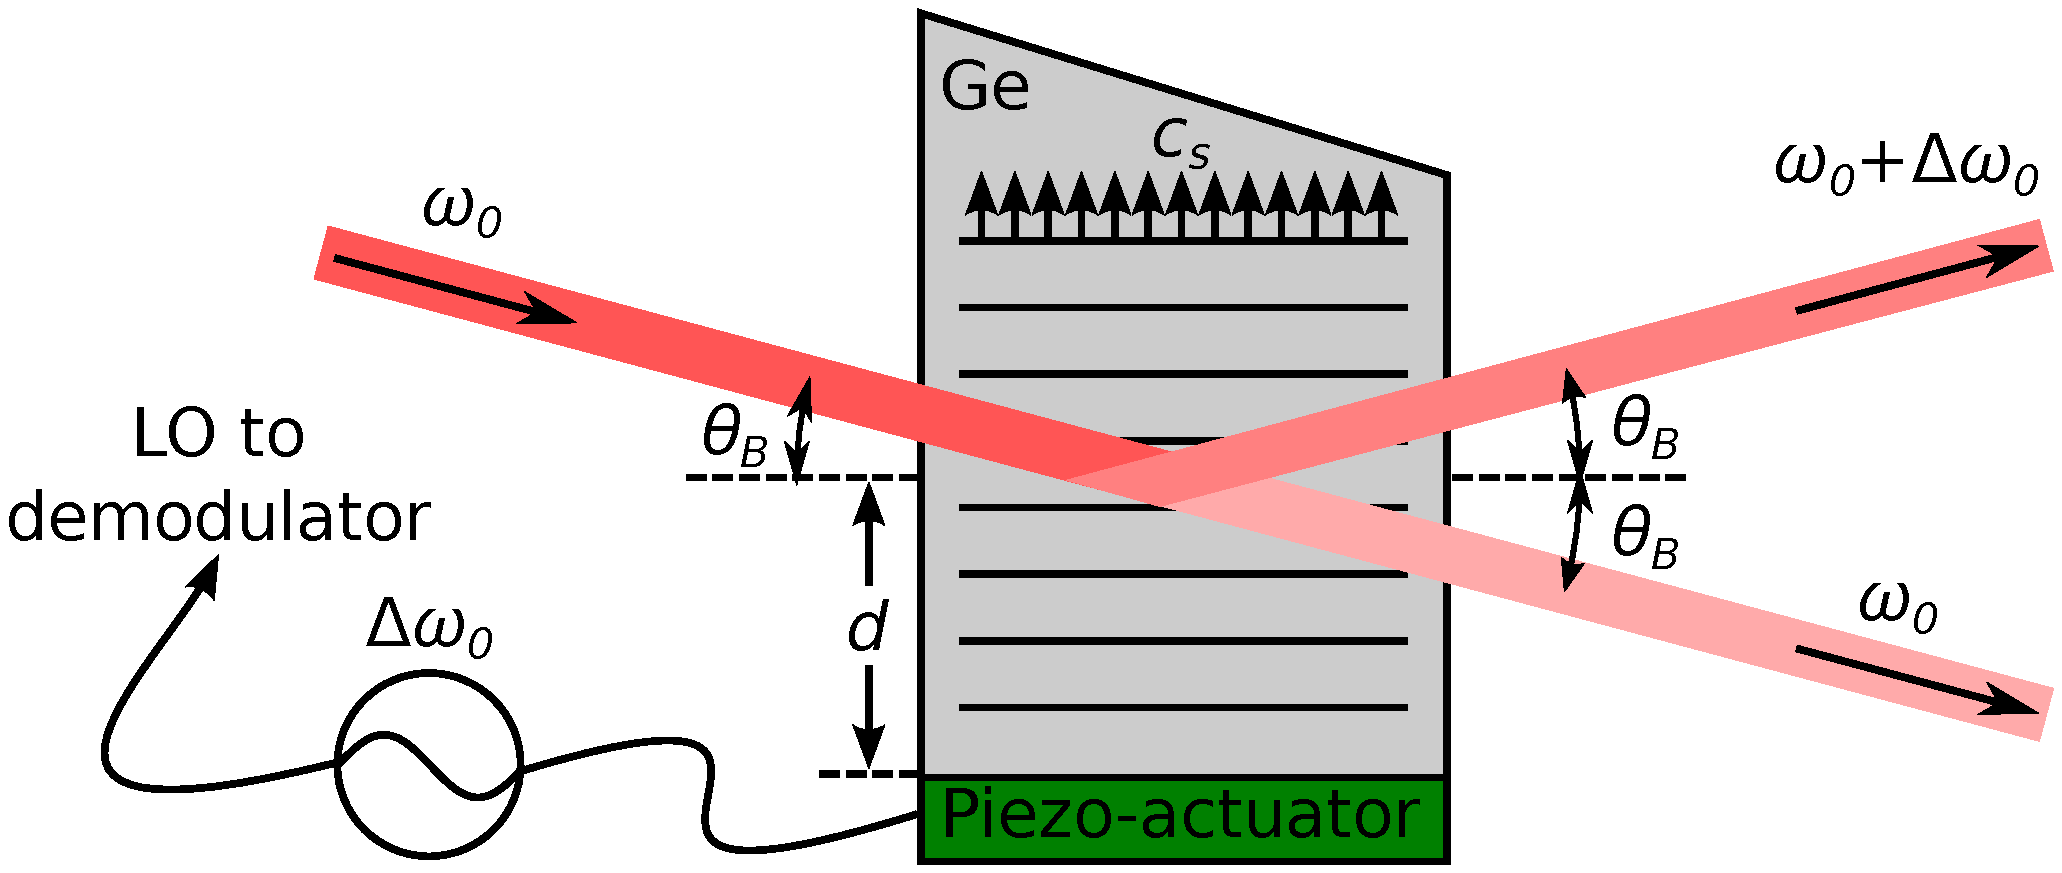
\includegraphics[width = \textwidth]{%
    Chapters/DesignConsiderations/figs/aom_scattering_diagram.pdf}
  \caption[Illustration of AOM operation in a heterodyne interferometer]{%
    An illustration of AOM operation in a heterodyne interferometer.
    A piezo-actuator drives sound waves of angular frequency $\Delta \omega_0$
    through a crystal (usually Germanium for $\SI{10.6}{\micro\meter}$ light),
    and these sound waves deflect and Doppler shift light
    that is incident upon the crystal at the Bragg angle $\theta_B$.
    The sound waves propagate from the piezo-actuator
    to the AOM's optically active region
    over finite time $\tau = d / c_s$.
    The RF waveform that drives the piezo-actuator
    is sampled and used to demodulate the heterodyne interference signal.
    Note that for simplicity the refraction of the beam
    as it enters and exits the crystal is \emph{not} depicted.}
\label{fig:DesignConsiderations:aom_scattering_diagram}
\end{figure}

The coupling of the AOM's drive signal to the deflected beam
occurs on the crystal's sound-wave timescale.
If the sound waves must propagate a distance $d$
from the piezo-actuator to the AOM's optically active region,
the drive signal is coupled to the deflected beam
only after time delay $\tau = d / c_s$.
The sound speed in Germanium is $c_s = \SI{5400}{\meter\per\second}$
such that a distance $d = \SI{1}{\centi\meter}$
is accompanied by a time delay $\tau = \SI{1.85}{\micro\second}$.
Note that this is large compared to many other timescales
typically considered in interferometry;
for example, light propagates
through $\SI{1}{\meter}$ of air
in only $\SI{3.33}{\nano\second}$,
and an RF signal propagates
through $\SI{1}{\meter}$ of RG-58 coaxial cable
(for which the index of refraction is $\sim 3 / 2$)
in only $\SI{5}{\nano\second}$.

In the presence of LO phase noise,
an AOM's finite coupling time
can degrade the performance of a heterodyne interferometer.
A local oscillator with phase noise is well-described by
\begin{equation}
  V_{\text{LO}}(t)
  =
  V_{0}
  e^{-i [\Delta \omega_0 t + \phi_{\Delta \omega_0}(t)]},
\end{equation}
where $\phi_{\Delta \omega_0}(t)$ is a zero-mean, stationary, random process
known as the LO's \emph{phase deviation}
whose temporal variation causes
the LO's instantaneous angular frequency
to wander about its nominal value $\Delta \omega_0$.
Then, to account for the AOM's finite coupling time and
the LO phase noise, take
$\Delta \omega_0 t
\rightarrow
[\Delta \omega_0 (t - \tau) + \phi_{\Delta \omega_0}(t - \tau)]$
in the heterodyne intensity
(\ref{eq:InterferometricMethods:heterodyne_intensity}).
Neglecting finite sampling-volume effects,
the heterodyne output voltage from a given detector element
is simply proportional to the local intensity, i.e.\
\begin{align}
  \begin{aligned}
    V_{\text{het}}(t)
    &=
    2 V_0
    \bigl\{%
      1
      +
      \cos\left[%
        \Delta \omega_0 t
        +
        \bar{\phi}_{\text{eff}}
        +
        \phi_{\Delta \omega_0}(t - \tau)
      \right]
      \\
      &\quad-
      \tilde{\phi}(x_{\image}, t)
      \sin\left[%
        \Delta \omega_0 t
        +
        \bar{\phi}_{\text{eff}}
        +
        \phi_{\Delta \omega_0}(t - \tau)
      \right]
    \bigr\},
  \end{aligned}
\end{align}
where $\bar{\phi}_{\text{eff}} = \bar{\phi} - \Delta \omega_0 \tau$.
Then, taking inspiration from the demodulated optical intensities
(\ref{eq:InterferometricMethods:heterodyne_interferometer_I_and_Q_intensity}),
the demodulated in-phase ($V_I$) and quadrature ($V_Q$) voltages are defined as
\begin{align}
  V_{I}(t)
  +
  i \cdot V_{Q}(t)
  &=
  \frac{1}{V_0}
  \langle
    V_{\text{LO}}(t)
    \cdot
    V_{\text{het}}(t)
  \rangle_{\Delta \omega_0}
  \notag \\
  &=
  V_0
  e^{i \bar{\phi}_{\text{eff}}}
  \left[
    1
    +
    i \tilde{\phi}_m(x_{\image}, t)
  \right],
  \label{eq:DesignConsiderations:heterodyne_interferometer_I_and_Q_voltage}
\end{align}
where
\begin{align}
  \tilde{\phi}_m(x_{\image}, t)
  &=
  \tilde{\phi}(x_{\image}, t)
  +
  \delta \phi_{\Delta \omega_0}(t, -\tau),
  \label{eq:DesignConsiderations:measured_phase_with_LO_phase_noise}
  \\
  \delta \phi_{\Delta \omega_0}(t, \tau)
  &=
  \phi_{\Delta \omega_0}(t + \tau)
  -
  \phi_{\Delta \omega_0}(t).
\end{align}
The quantity $\delta \phi_{\Delta \omega_0}(t, \tau)$
is referred to as the ``instrumental phase noise'', and
it is produced by the modulator's finite coupling time $\tau$ and
the LO's phase deviation $\phi_{\Delta \omega_0}(t)$.
Typically, $|\delta \phi_{\Delta \omega_0}(t, \tau)| \ll 1$, and
only terms to first order in $\delta \phi_{\omega_0}$ and $\tilde{\phi}$
were retained in the demodulated voltages
(\ref{eq:DesignConsiderations:heterodyne_interferometer_I_and_Q_voltage}).
Comparing
(\ref{eq:DesignConsiderations:heterodyne_interferometer_I_and_Q_voltage})
with the demodulated intensities
(\ref{eq:InterferometricMethods:heterodyne_interferometer_I_and_Q_intensity}),
one readily sees that
the \emph{measured} phase fluctuation is $\tilde{\phi}_m$ defined in
(\ref{eq:DesignConsiderations:measured_phase_with_LO_phase_noise});
that is, the fluctuating signal is contaminated
by the instrumental phase noise.
The spectral properties of $\delta \phi_{\Delta\omega_0}(t, \tau)$
are thoroughly discussed in Appendix~\ref{app:OscillatorPhaseNoise}.
As $\delta \phi_{\omega_0}(t, \tau)$ and
$\tilde{\phi}(x_{\image}, t)$ are uncorrelated,
the one-sided autospectral density of the measured phase fluctuations is
\begin{equation}
    G_{\tilde{\phi}_m,\tilde{\phi}_m}(f)
    =
    G_{\tilde{\phi},\tilde{\phi}}(f)
    +
    8 \sin^2(\pi f \tau) \mathcal{L}_{\Delta\omega_0}(f),
\end{equation}
where
$G_{\tilde{\phi},\tilde{\phi}}(f)$ is the \emph{true}
one-sided autospectral density of the phase fluctuation $\tilde{\phi}$ and
$\mathcal{L}_{\Delta\omega_0}(f)$ is the phase noise of the LO,
as defined in Appendix~\ref{app:OscillatorPhaseNoise}.


\section{Amplitude noise: sources \& effects}
\label{sec:DesignConsiderations:amplitude_noise}
Detector noise and shot noise are typically
the largest contributors to amplitude noise
in the heterodyne interference signal, while
a noisy amplifier can degrade the signal-to-noise ratio.
The demodulation of such amplitude noise
is throughly discussed by Rakhmanov in~\cite{rakhmanov_ao01}.
While Rakhmanov does not explicitly consider quadrature heterodyne detection,
his results can be naturally applied to quadrature heterodyne detection,
as is done below.


\subsection{Detector noise}
Real-world detector operation is associated with intrinsic noise.
This noise results from, among other things,
Johnson thermal noise in the detector and
shot noise in the background radiation flux
\cite{hamamatsu_ir_detectors}.
A detector's noise is often characterized by
its noise-equivalent power ($NEP$):
when the power of the incident optical signal is equal to the $NEP$,
the signal-to-noise ratio is unity.
Consider optical power $\delta P(t)$ that, when incident upon a detector,
produces a signal that
emulates the statistical properties of the detector noise
(e.g.\ $\delta P(t)$ is a real-valued, zero-mean, stationary, random process).
Then, the $NEP$ corresponds to the root mean square (RMS) of $\delta P(t)$,
and
\begin{equation}
  (NEP)^2
  =
  \int_{\Delta f}
  G_{\delta P, \delta P}(f) df,
  \label{eq:DesignConsiderations:NEP_from_spectral_density}
\end{equation}
where $G_{\delta P, \delta P}(f)$ is
the one-sided autospectral density of $\delta P(t)$ and
the integral is performed over the temporal bandwidth $\Delta f$
of the desired measurement.
Note that $G_{\delta P, \delta P}(f)$ depends on both
extensive (e.g.\ element area) and intensive (e.g.\ element material)
properties of the detector.
To more easily compare detectors of different sizes and materials,
the $NEP$ of a given detector is often parameterized as
\begin{equation}
  NEP = \frac{\sqrt{A \cdot \Delta f}}{D^{*}},
  \label{eq:DesignConsiderations:NEP_from_engineering_parameters}
\end{equation}
where $A$ is the effective area of the detector element,
$\Delta f$ is the temporal bandwidth of the desired measurement, and
$D^{*}$ is the detector's specific detectivity~\cite{jones_josa60}.
Note that larger $D^{*}$ corresponds to increased detector sensitivity.
If $G_{\delta P, \delta P}(f)$ is approximately constant
over the bandwidth $\Delta f$, then equating
(\ref{eq:DesignConsiderations:NEP_from_spectral_density})
to the square of
(\ref{eq:DesignConsiderations:NEP_from_engineering_parameters})
yields
\begin{equation}
  G_{\delta P, \delta P}(f)
  =
  \frac{A}{(D^*)^2}.
  \label{eq:DesignConsiderations:NEP_spectral_density}
\end{equation}

It is now shown shown that
signal demodulation pushes detector noise
near the heterodyne angular frequency $\Delta \omega_0$
into the baseband signal.
Taking inspiration from the demodulated optical intensities
(\ref{eq:InterferometricMethods:heterodyne_interferometer_I_and_Q_intensity}),
define the total $NEP$ contamination of
the in-phase ($I$) and quadrature ($Q$) signals to be
\begin{align}
  \delta P_{IQ}(t)
  =
  \frac{2 \sqrt{2}}{\pi}
  e^{- i \Delta \omega_0 t} \cdot \delta P(t).
  \label{eq:DesignConsiderations:demodulated_NEP_complex}
\end{align}
Here, the demodulated noise has \emph{not} yet been low-pass filtered.
The autocorrelation function of the demodulated noise is
\begin{align}
  R_{\delta P_{IQ},\delta P_{IQ}}(\tau)
  &=
  E\left[\delta P_{IQ}(t) \cdot \delta P_{IQ}^*(t + \tau) \right]
  \notag \\
  &=
  \frac{8}{\pi^2}
  \cdot
  e^{i \Delta \omega_0 \tau}
  \cdot
  R_{\delta P, \delta P}(\tau),
\end{align}
where $z^*$ indicates the complex conjugate of $z$ and
$R_{\delta P, \delta P}(\tau)$ is the
autocorrelation function of the $NEP$.
The autospectral density of the demodulated noise is then
\begin{align}
  S_{\delta P_{IQ},\delta P_{IQ}}(f)
  &=
  \mathcal{F}\left[ R_{\delta P_{IQ},\delta P_{IQ}}(\tau) \right](f)
  \notag \\
  &=
  \frac{8}{\pi^2}
  \cdot
  \mathcal{F}\left[
    e^{i 2 \pi \Delta f_0 \tau} \cdot R_{\delta P, \delta P}(\tau)
  \right](f)
  \notag \\
  &=
  \frac{8}{\pi^2}
  \cdot
  S_{\delta P, \delta P}(f + \Delta f_0),
\end{align}
where
$\Delta f_0 = \Delta \omega_0 / (2 \pi)$ is the heterodyne frequency and
$S_{\delta P, \delta P}(f)$ is the autospectral density of the $NEP$.
The demodulated signals are typically low-pass filtered
such that only the desired information at $|f| \ll \Delta f_0$
survives
\begin{equation}
  \left.
    S_{\delta P_{IQ},\delta P_{IQ}}(f)
  \right|_{|f| \ll \Delta f_0}
  \approx
  \frac{8}{\pi^2}
  \cdot
  S_{\delta P, \delta P}(\Delta f_0).
  \label{eq:DesignConsiderations:detector_noise_demodulated}
\end{equation}
Thus, the $NEP$ at the heterodyne frequency $\Delta f_0$
is pushed into the baseband signal via the demodulation process.
Note that the autospectral density of the demodulated detector noise
(\ref{eq:DesignConsiderations:detector_noise_demodulated})
is in agreement with the literature
(e.g.\ see Rakhmanov's Eq.~(47) in~\cite{rakhmanov_ao01}
with $d_1 = 2 / \pi$ for demodulation against
the \emph{first harmonic} of a zero-mean square wave
with frequency $\Delta f_0$ and peak-to-peak amplitude of two;
see Section~\ref{sec:DesignConsiderations:demodulation:nonideal_mixing}
for the physical significance of demodulation against such a square wave).
The corresponding one-sided autospectral density
of the demodulated detector noise is
\begin{align}
  \left.
    G_{\delta P_{IQ},\delta P_{IQ}}(f)
  \right|_{|f| \ll \Delta f_0}
  &\approx
  \frac{8}{\pi^2}
  \cdot
  G_{\delta P, \delta P}(\Delta f_0).
  \notag \\
  &=
  \frac{8}{\pi^2}
  \cdot
  \frac{A}{(D^*)^2},
  \label{eq:DesignConsiderations:demodulated_NEP_spectral_density}
\end{align}
where the last line follows from
(\ref{eq:DesignConsiderations:NEP_spectral_density}) and
the assumption that $D^{*}$ is the specific detectivity
for frequencies $f$ in the neighborhood
of the heterodyne frequency $\Delta f_0$.


\subsection{Shot noise}
The discrete nature of the arriving photons results in shot noise.
Well-modeled as a Poisson process,
the shot noise increases as $N_{\gamma}^{1/2}$, where
$N_{\gamma}$ is the number of incident photons.
Because the incident optical power (and hence the number of incident photons)
in the heterodyne optical signal is modulated as a function of time,
the corresponding shot noise is inherently nonstationary.
Surprisingly, however, the demodulated shot noise \emph{is} stationary
(e.g.\ see Rakhmanov's Eq.~(59) in~\cite{rakhmanov_ao01}).
Note that Rakhmanov only considers \emph{one} of the demodulated signals, and
maximizing the signal-to-noise ratio in the demodulated signal
requires careful selection of the local oscillator's phase
relative to that of the heterodyne signal
(he terms this the ``demodulation phase'' and
represents it via $\gamma$).
However, by employing quadrature heterodyne detection~\cite{carlstrom_rsi88},
in which $\gamma_Q = \gamma_I + \pi / 2$,
the total shot-noise contamination $\delta P_{IQ}$
of the in-phase ($I$) and quadrature ($Q$) signals
(with $\delta P_{IQ}$ as defined in
(\ref{eq:DesignConsiderations:demodulated_NEP_complex}),
but with $\delta P$ now corresponding to the shot-noise optical power)
is \emph{independent} of the demodulation phase, i.e.\
\begin{align}
  \left.
    S_{\delta P_{IQ}, \delta P_{IQ}}(f)
  \right|_{|f| \ll \Delta f_0}
  &=
  \frac{8}{\pi^2}
  \cdot
  h f_0 P_0,
\end{align}
where
$h$ is the Planck constant,
$f_0$ is the frequency of the incident photons, and
$P_0$ is the DC optical power impinging upon the detector.
The corresponding one-sided autospectral density is
\begin{align}
  \left.
    G_{\delta P_{IQ}, \delta P_{IQ}}(f)
  \right|_{|f| \ll \Delta f_0}
  =
  \frac{16}{\pi^2}
  \cdot
  h f_0 P_0.
  \label{eq:DesignConsiderations:demodulated_shot_noise_spectral_density}
\end{align}
Rakhmanov notes that
(\ref{eq:DesignConsiderations:demodulated_shot_noise_spectral_density})
corresponds to the well-known Schottky formula.


\subsection{Amplifier noise}
The noise \emph{factor} $F$ of an RF amplifier is defined as the ratio of
the signal-to-noise ratio at the device's input ($SNR_{\text{in}}$) to
the signal-to-noise ratio at the device's output ($SNR_{\text{out}}$)
\begin{equation}
  F = \frac{SNR_{\text{in}}}{SNR_{\text{out}}};
\end{equation}
often, the noise factor $F$ is given
in terms of the noise \emph{figure} $NF$
\cite{minicircuits_amplifier_terms_defined}
\begin{equation}
  NF = 10 \log_{10} F.
\end{equation}
If several amplifiers are cascaded,
the total noise factor of the amplifier chain
can be computed using the well-known Friis noise-factor formula.
Note that the noise factor is only defined
in the context of a signal-to-noise ratio, so
it is not conventional to write down the corresponding
autospectral density of the amplifier noise in absolute units.


\section{Demodulation}
\label{sec:DesignConsiderations:demodulation}
The heterodyne interferometer's IF signal must be demodulated
in order to recover the baseband phase information.
Demodulation is typically described as an analog process
in which the IF signal is \emph{mixed} with a local oscillator (LO), but
demodulation can also be performed digitally
\cite{vanzeeland_rsi08, mlynek_fst12} or
with non-mixer-based analog electronics~\cite{mlynek_rsi17}.
The focus here, however, is on the analog, mixer-based approach.
Section~\ref{sec:DesignConsiderations:demodulation:ideal}
describes ideal analog demodulation.
Sections~\ref{sec:DesignConsiderations:demodulation:nonideal_mixing} and
\ref{sec:DesignConsiderations:demodulation:demodulator_imbalances}
discuss nonideal aspects of analog mixers and demodulators, and
Section~\ref{sec:DesignConsiderations:demodulation:imperfection_implications}
analyzes the implications of these imperfections
in the context of fluctuation measurements.


\subsection{Ideal demodulation}
\label{sec:DesignConsiderations:demodulation:ideal}
A typical analog $I\&Q$ demodulator consists of
a $90^{\circ}$ splitter,
two double-balanced mixers, and
a $0^{\circ}$ splitter~\cite{minicircuits_modulators}, as shown in
Fig.~\ref{fig:DesignConsiderations:analog_IQ_demodulator}(a).
The $90^{\circ}$ splitter divides the incident local oscillator (LO) signal
\begin{equation}
  \text{LO}(t) = \frac{4 \sqrt{2}}{\pi} \cos(\Delta\omega_0 t)
\end{equation}
into an ``in-phase'' copy of the LO
\begin{equation}
  \text{LO}_0(t)
  =
  \frac{4}{\pi} \cos(\Delta\omega_0 t)
\end{equation}
and a $\pi / 2$ phase-advanced copy of the LO
\begin{equation}
  \text{LO}_{\pi / 2}(t)
  =
  \frac{4}{\pi} \cos\left( \Delta\omega_0 t + \frac{\pi}{2} \right)
  =
  -\frac{4}{\pi} \sin(\Delta\omega_0 t).
\end{equation}
Note that the power (i.e.\ the mean-square value) in the incident LO signal
is split evenly between $\text{LO}_0(t)$ and $\text{LO}_{\pi / 2}(t)$.
Further, the normalization of $\text{LO}_0(t)$ and $\text{LO}_{\pi / 2}(t)$
is motivated by and is consistent with the physical processes
that occur in a typical ring-diode double-balanced mixer, as discussed in
Section~\ref{sec:DesignConsiderations:demodulation:nonideal_mixing}.
The $0^{\circ}$ splitter divides the intermediate frequency (IF) signal
\begin{equation}
  \text{IF}(t) = A_{\text{IF}} \cos(\Delta\omega_0 t + \phi)
  \label{eq:DesignConsiderations:IF_perfect_sinusoid}
\end{equation}
into two identical copies of the IF
\begin{equation}
  \text{IF}_0(t)
  =
  \frac{A_{\text{IF}}}{\sqrt{2}} \cos(\Delta\omega_0 t + \phi).
  \label{eq:DesignConsiderations:split_IF}
\end{equation}
Like the LO signal, the power in the incident IF signal
is split evenly between the two copies.
The signal at the demodulator's in-phase ($I$) port
then corresponds to the product of
$\text{IF}_0(t)$ with the in-phase LO signal $\text{LO}_0(t)$:
\begin{equation}
  \text{LO}_0(t) \cdot \text{IF}_0(t)
  =
  \frac{\sqrt{2} A_{\text{IF}}}{\pi}
  \left[
    \cos(\phi) + \cos(2 \Delta\omega_0 t + \phi)
  \right].
\end{equation}
Such signal multiplication is often referred to as ``mixing''.
Low-pass filtering the signal exiting the demodulator's $I$ port
yields the baseband in-phase signal
\begin{equation}
  I = \frac{\sqrt{2} A_{\text{IF}}}{\pi} \cos\phi.
\end{equation}
Similar reasoning regarding the product
$\text{LO}_{\pi / 2}(t) \cdot \text{IF}_0(t)$
at the demodulator's quadrature ($Q$) port
yields the baseband quadrature signal
\begin{equation}
  Q = \frac{\sqrt{2} A_{\text{IF}}}{\pi} \sin\phi.
\end{equation}
Note that the total power $I^2 + Q^2$ in the $I\&Q$ signals
is $\SI{4}{\decibel}$ lower
than the power in the incident IF signal.
This is known as the \emph{conversion loss} of the demodulator;
real-world demodulators will have larger conversion losses
due to dissipation and other nonideal effects.
An \emph{absolute} phase measurement $\phi_m$ is then obtained via
\begin{equation}
  \phi_m = \atantwo\left(Q, I\right),
  \label{eq:DesignConsiderations:phase_from_arctangent}
\end{equation}
where $\atantwo\left(Q, I\right)$
is the arctangent function of two arguments, which
uses the signs of $Q$ and $I$ to correctly determine
the quadrant corresponding to the tangent of $Q / I$.
Note that in the ideal case the measured phase is
equal to the true phase, i.e.\ $\phi_m = \phi$, and
that $\phi_m$ is independent of the power in the incident IF signal.

\begin{figure}
  \centering
  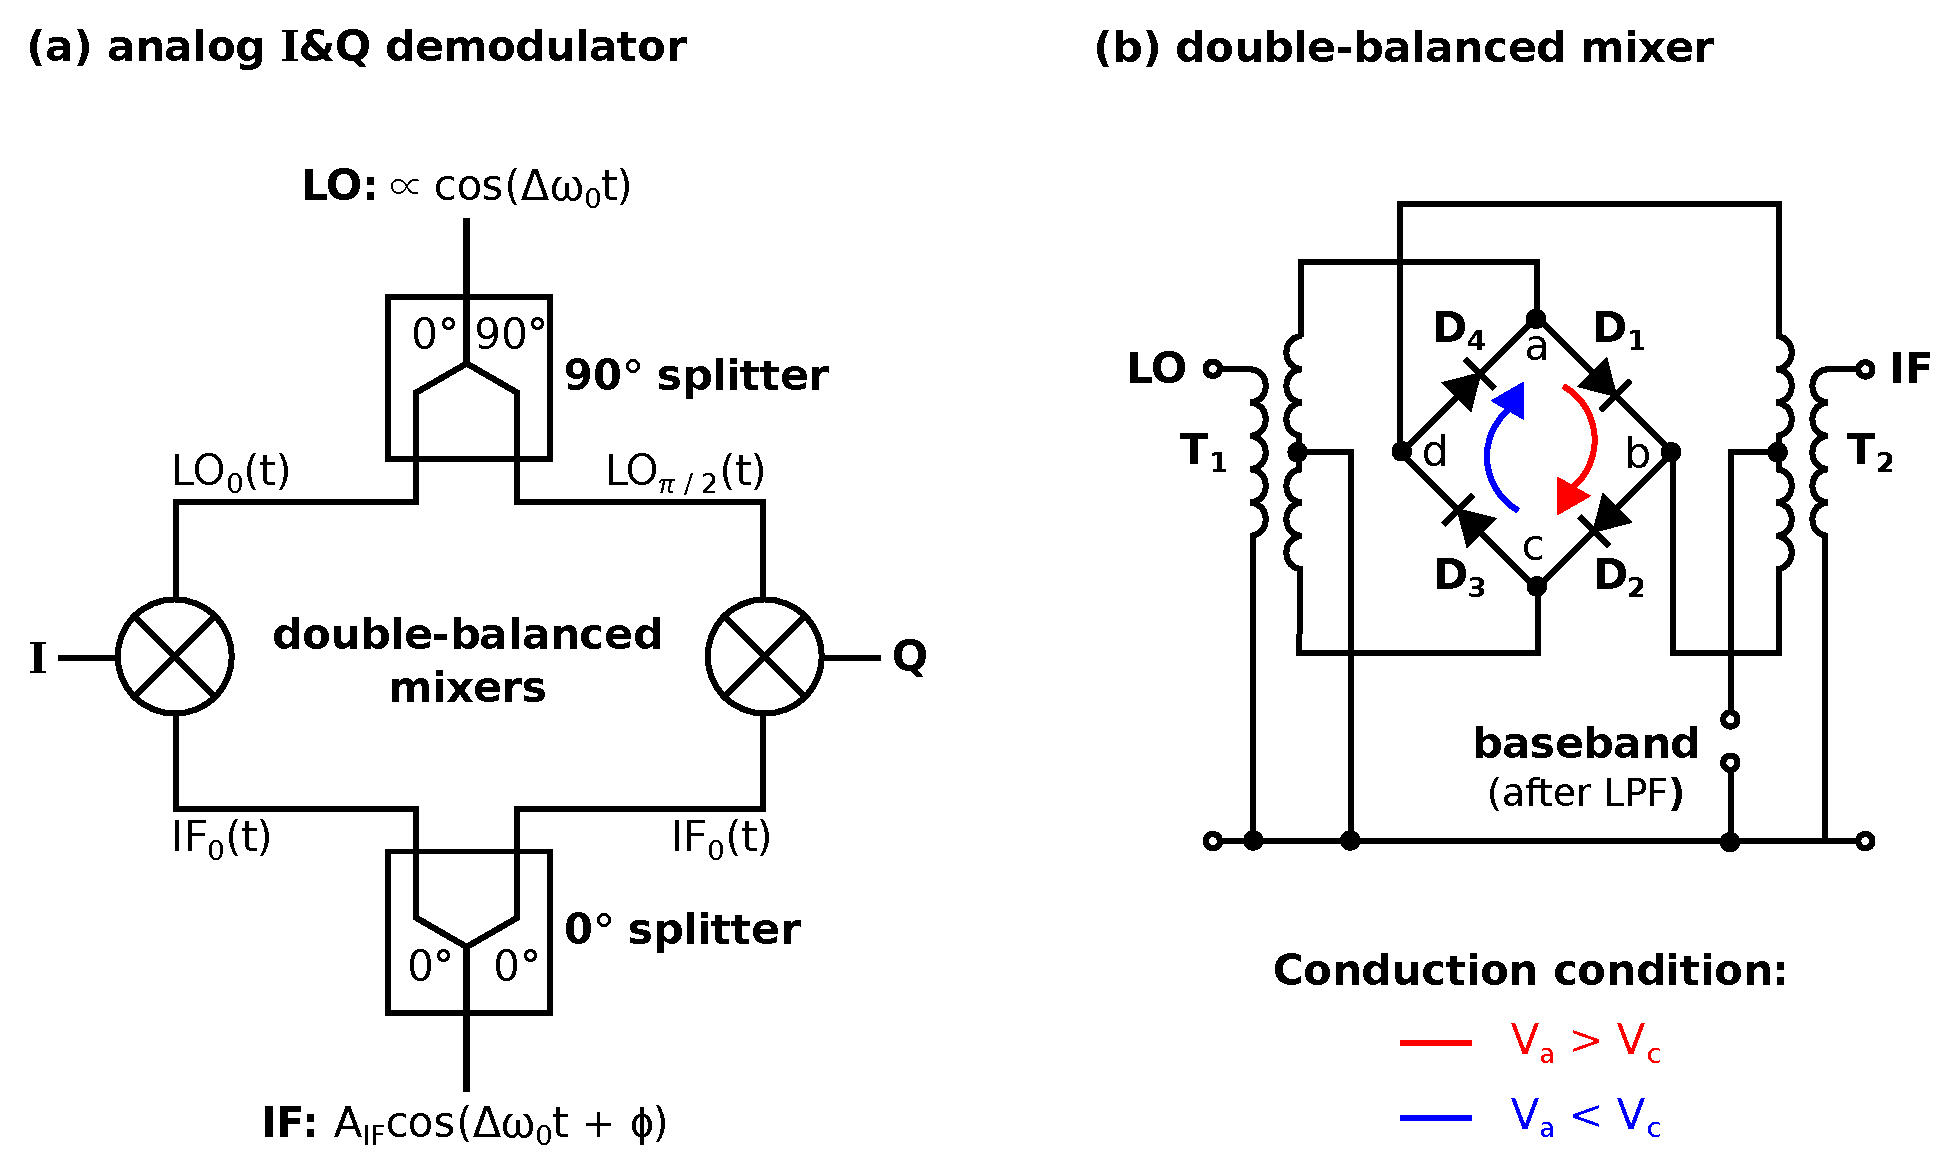
\includegraphics[width = \textwidth]{%
    Chapters/DesignConsiderations/figs/analog_IQ_demodulator.pdf}
  \caption[Components of a typical analog $I\&Q$ demodulator]{%
    (a) A typical analog $I\&Q$ demodulator and
    (b) a typical diode-ring double-balanced mixer.}
  \label{fig:DesignConsiderations:analog_IQ_demodulator}
\end{figure}


\subsection{Nonideal mixing}
\label{sec:DesignConsiderations:demodulation:nonideal_mixing}
In Section~\ref{sec:DesignConsiderations:demodulation:ideal},
mixing was idealized as the multiplication of the IF signal
by a sinusoidal LO signal.
However, in practice, more complex processes are used
to maximize the mixer's linear dynamic range and minimize its noise figure
\cite{analog_devices_mix_and_mod,bryant_mult_vs_mod}.

For example, a typical ring-diode double-balanced mixer
\cite{analog_devices_mix_and_mod}
is shown in Fig.~\ref{fig:DesignConsiderations:analog_IQ_demodulator}(b).
The balun transformers $T_1$ and $T_2$
isolate the baseband port from the LO and IF ports.
Typically, the LO power is $\sim \SI{20}{\deci\bel}$ larger than the IF power.
As a result, the LO alone is responsible
for biasing the mixer's diodes into conduction.
Note that the diodes are not all simultaneously biased into conduction.
Instead, when $V_a > V_c$ (neglecting the diode drops),
diodes $D_1$ and $D_2$ are forced into conduction such that
$V_b$ acts as a virtual ground for the IF signal
coupled through transformer $T_2$.
Then, when the LO changes sign such that $V_a < V_c$,
diodes $D_1$ and $D_2$ stop conducting, and
diodes $D_3$ and $D_4$ begin to conduct,
forcing the virtual ground to jump from $V_b$ to $V_d$.
Thus, the ring diode acts as a switch
for the polarization of the coupled IF signal,
with the switching governed by the sign and frequency of the LO.
Low-pass filtering the polarization-modulated IF, of course,
yields the desired baseband signal.
Note that the diode switching time should be minimized
for optimal modulation,
explaining why some manufacturers
advocate the use of a square, rather than a sinusoidal, LO
\cite{minicircuits_mixer_faqs}.

This polarization modulation can alter the baseband spectrum.
To see this, note that the sign of the in-phase LO signal
is simply a zero-mean square wave with even symmetry about the origin,
as shown in the lower pane of
Fig.~\ref{fig:DesignConsiderations:LO_switching_function}.
The Fourier series of such a square wave
consists of a sum over all of the LO's \emph{odd} harmonics:
\begin{align}
  \text{sgn}\left( \text{LO}_0(t) \right)
  &=
  \frac{4}{\pi}
  \sum_{n = 1}^{\infty}
  \frac{(-1)^{n - 1}}{2n - 1} \cos[(2n - 1) \Delta\omega_0 t]
  \\
  &\begin{aligned}
    =
    \frac{4}{\pi}
    \biggl[%
      \cos(\Delta\omega_0 t)
      &-
      \frac{1}{3} \cos(3 \Delta\omega_0 t)
      +
      \cdots
    \biggr].
  \end{aligned}
  \notag
\end{align}
Now, if the IF signal is a perfect sinusoid
as in (\ref{eq:DesignConsiderations:IF_perfect_sinusoid}),
following Section~\ref{sec:DesignConsiderations:demodulation:ideal}'s program
of mixing the LO with the IF and low-pass filtering yields
the desired in-phase baseband signal, e.g.\
\begin{align}
  I
  &=
  \bigl[%
    \text{sgn}\left( \text{LO}_0(t) \right)
    \cdot
    \text{IF}_0(t)
  \bigr]
  \biggr|_{|\omega| \ll \Delta\omega_0}
  \notag \\
  &=
  \frac{\sqrt{2} A_{\text{IF}}}{\pi} \cos\phi
\end{align}
However, if the path from the mixer's IF port to its baseband port
is not wholly linear
(and every real-world device exhibits \emph{some} degree of nonlinearity),
the IF signal will contain contributions from its higher-order harmonics.
If this nonlinearity depends only on the magnitude of the IF
(e.g.\, double-sided saturation/clipping of the signal),
only the odd harmonics of the fundamental will contribute, i.e.\
\begin{equation}
  \text{IF}_0(t)
  =
  \frac{1}{\sqrt{2}}
  \sum_{n = 1}^{\infty}
  A_{2n - 1} \cos\left[ (2n - 1) (\Delta\omega_0 t + \phi) \right],
\end{equation}
where $A_n / \sqrt{2}$ is the Fourier coefficient of the $n\ts{th}$ harmonic
(note that this unconventional normalization facilitates comparison with
the previous, ideal definition of $IF_0(t)$
(\ref{eq:DesignConsiderations:split_IF})).
Typically, $A_n$ decreases as $n$ increases, but
raising the IF amplitude drives more nonlinear interactions and
increases the power in the higher order harmonics relative to the fundamental.
Then,
following Section~\ref{sec:DesignConsiderations:demodulation:ideal}'s program
of mixing the LO with the IF and low-pass filtering yields
\begin{align}
  I
  &=
  \bigl[%
    \text{sgn}\left( \text{LO}_0(t) \right)
    \cdot
    \text{IF}_0(t)
  \bigr]
  \biggr|_{|\omega| \ll \Delta\omega_0}
  \notag \\
  &=
  \frac{\sqrt{2} A_1}{\pi}
  \left[%
    \cos\phi
    -
    \frac{1}{3}\left( \frac{A_3}{A_1} \right) \cos 3 \phi
    +
    \cdots
  \right].
\end{align}
That is, the higher order harmonics of the IF signal
interact with the corresponding higher order harmonics
of the LO switching function
to produce harmonics in the baseband signal.
The coefficient $A_n / (n \cdot A_1)$ gives
the \emph{suppression} of the $n\ts{th}$ harmonic, and
it is typically expressed in decibels
referenced to the power of the carrier, or dBc, as
\begin{equation}
  \text{suppression of $n\ts{th}$ harmonic [dBc]}
  =
  20 \log_{10} \left( \frac{A_n}{n \cdot A_1} \right).
\end{equation}
Noting that $\text{sgn}(\text{LO}_{\pi / 2}(t))$
is an inverted, zero-mean square wave
with \emph{odd} symmetry about the origin,
as shown in the lower pane of
Fig.~\ref{fig:DesignConsiderations:LO_switching_function},
a similar path of reasoning to that used above
shows that the quadrature baseband signal is
\begin{align}
  Q
  &=
  \bigl[%
    \text{sgn}\left( \text{LO}_{\pi / 2}(t) \right)
    \cdot
    \text{IF}_0(t)
  \bigr]
  \biggr|_{\omega \ll \Delta\omega_0}
  \notag \\
  &=
  \frac{\sqrt{2} A_1}{\pi}
  \left[%
    \sin\phi
    +
    \frac{1}{3}\left( \frac{A_3}{A_1} \right) \sin 3 \phi
    +
    \cdots
  \right].
\end{align}
Additional distortion of the baseband signal results
if the IF power becomes comparable the LO power,
say within $\SI{10}{\deci\bel}$,
as the IF signal begins to contribute
to the modulation of the diode conduction.

\begin{figure}
  \centering
  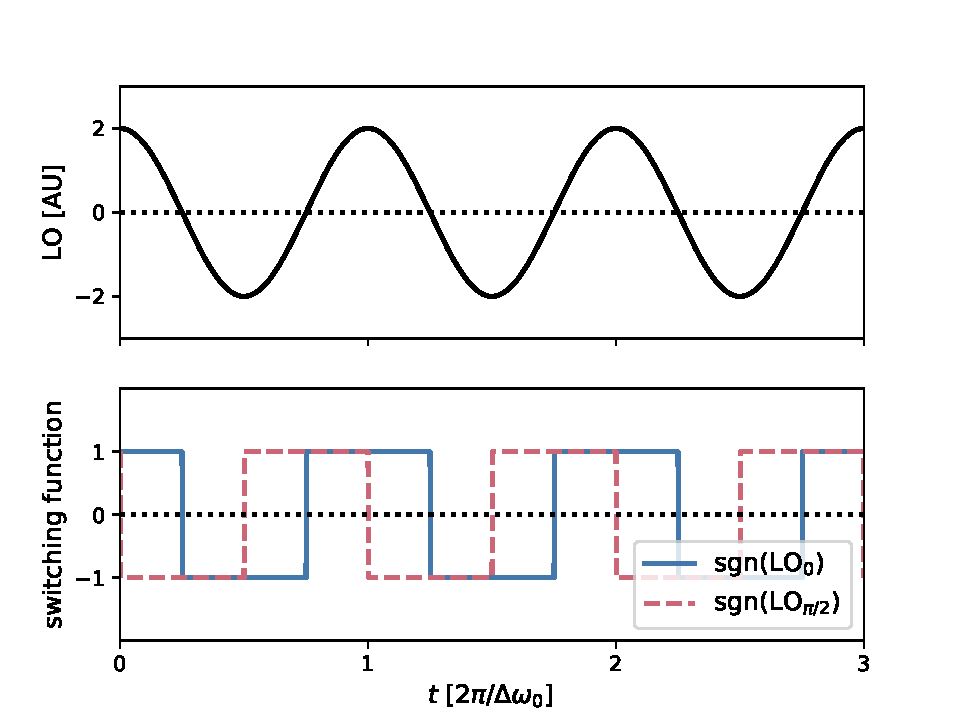
\includegraphics[width = \textwidth]{%
    Chapters/DesignConsiderations/figs/LO_switching_function.pdf}
  \caption[LO switching functions]{%
    The LO switching functions.
    The top panel displays the incident sinusoidal LO signal, while
    the bottom panel shows the \emph{sign} of
    the in-phase ($\text{LO}_0$) and
    the $\pi / 2$ phase-advanced ($\text{LO}_{\pi / 2}$)
    copies of the LO signals.}
  \label{fig:DesignConsiderations:LO_switching_function}
\end{figure}

Finally, the diodes of the mixers should be matched as closely as possible.
If, for example, diodes $D_1$ and $D_2$
have slightly different voltage drops than diodes $D_3$ and $D_4$,
the virtual grounds at $V_b$ and $V_d$ are not equivalent
when referenced to ground, and
the resulting baseband signal will have a DC offset.
With precision fabrication, however,
it is not uncommon for the DC offset to be smaller than $1\%$
of the amplitude of the baseband fundamental harmonic.


\subsection{Demodulator imbalances}
\label{sec:DesignConsiderations:demodulation:demodulator_imbalances}
In addition to two double-balanced mixers,
an analog $I\&Q$ demodulator also relies on
a $90^{\circ}$ splitter and a $0^{\circ}$ splitter.
Imbalances between any of these components
can result in imbalances in the baseband $I\&Q$ signals.
For example, unequal power division in the splitters
produces amplitude imbalances in the baseband $I\&Q$ signals, while
deviations from the nominal splitter phasings
produces phase imbalances in the baseband $I\&Q$ signals.
As discussed in
Section~\ref{sec:DesignConsiderations:demodulation:nonideal_mixing},
each double-balanced mixer can produce
spectral distortion and DC offsets in the baseband signal;
in addition, differences between the two mixers
can exacerbate amplitude and phase imbalances
in the baseband $I\&Q$ signals.
Taken all together, then,
the most general form for the baseband $I\&Q$ signals is
\begin{align}
  I
  &=
  I_1 \left\{%
    \cos\phi
    -
    \frac{I_3}{3 I_1}
    \cos \left( 3 \phi \right)
    +
    \cdots
  \right\}
  +
  \delta I,
  \label{eq:DesignConsiderations:I_general}
  \\
  Q
  &=
  Q_1 \left\{%
    \sin \left( \phi + \delta \right)
    +
    \frac{Q_3}{3 Q_1}
    \sin \left[ 3 \left( \phi + \delta \right) \right]
    +
    \cdots
  \right\}
  +
  \delta Q,
  \label{eq:DesignConsiderations:Q_general}
\end{align}
where
$I_1$ is the amplitude of the in-phase signal's fundamental harmonic,
$I_3$ is the amplitude of the in-phase signal's third harmonic, and
$\delta I$ is the in-phase signal's DC offset.
Similar nomenclature applies to the quadrature signal.
The phase imbalance of the demodulator is $\delta$.
Amplitude imbalances occur when $I_1 \neq Q_1$.
The harmonic suppressions are typically comparable,
e.g.\ $|I_3 / I_1| \approx |Q_3 / Q_1|$.
Note that (\ref{eq:DesignConsiderations:I_general}) and
(\ref{eq:DesignConsiderations:Q_general})
generalize previous forms for the $I\&Q$ signals
\cite{vanzeeland_rsi04}.


\subsection{Effects of demodulator imperfections}
\label{sec:DesignConsiderations:demodulation:imperfection_implications}
Demodulator imperfections produce systematic errors
in the measured phase~\cite{vanzeeland_rsi04,kasten_masters}.
Specifically, if the $I\&Q$ signals suffer from imbalances and nonlinearities,
as shown in (\ref{eq:DesignConsiderations:I_general}) and
(\ref{eq:DesignConsiderations:Q_general}),
then the measured phase $\phi_m$ computed via the inverse tangent formula
(\ref{eq:DesignConsiderations:phase_from_arctangent})
will \emph{not} correspond to the true phase $\phi$, i.e.\
\begin{equation}
  \phi_m = \phi + \delta \phi,
\end{equation}
where $\delta\phi$ is the error in the measured phase.
The phase error is a complicated, periodic function of the true phase,
i.e.\ $\delta\phi = \delta\phi(\phi)$~\cite{vanzeeland_rsi04}.
For small phase fluctuations $|\tilde{\phi}| \ll 1$
about an equilibrium phase $\bar{\phi}$,
the error $\delta\tilde{\phi}$ in the measured fluctuating phase
is simply the \emph{change} in the total phase error
between $\bar{\phi}$ and $\bar{\phi} + \tilde{\phi}$
\cite{kasten_masters}:
\begin{equation}
  \delta\tilde{\phi}
  =
  \delta\phi(\bar{\phi} + \tilde{\phi}) - \delta\phi(\bar{\phi})
  \approx
  \left[%
    \left. \frac{d(\delta\phi)}{d\phi} \right|_{\bar{\phi}}
  \right] \tilde{\phi}.
\end{equation}
Thus, the \emph{relative} error in the measured fluctuating phase is
\begin{equation}
  \frac{\delta\tilde{\phi}}{\tilde{\phi}}
  =
  \left. \frac{d(\delta\phi)}{d\phi} \right|_{\bar{\phi}}.
  \label{eq:DesignConsiderations:relative_fluctuation_error}
\end{equation}
The $I\&Q$ Lissajous curves and
the relative errors in the measured fluctuating phase
that result from various demodulator imperfections
are displayed in
Fig.~\ref{fig:DesignConsiderations:effects_of_demodulator_imperfections}.
Obviously, each demodulator imperfection should be minimized
in order to minimize the relative error
in the measured fluctuating phase.

\begin{figure}
  \centering
  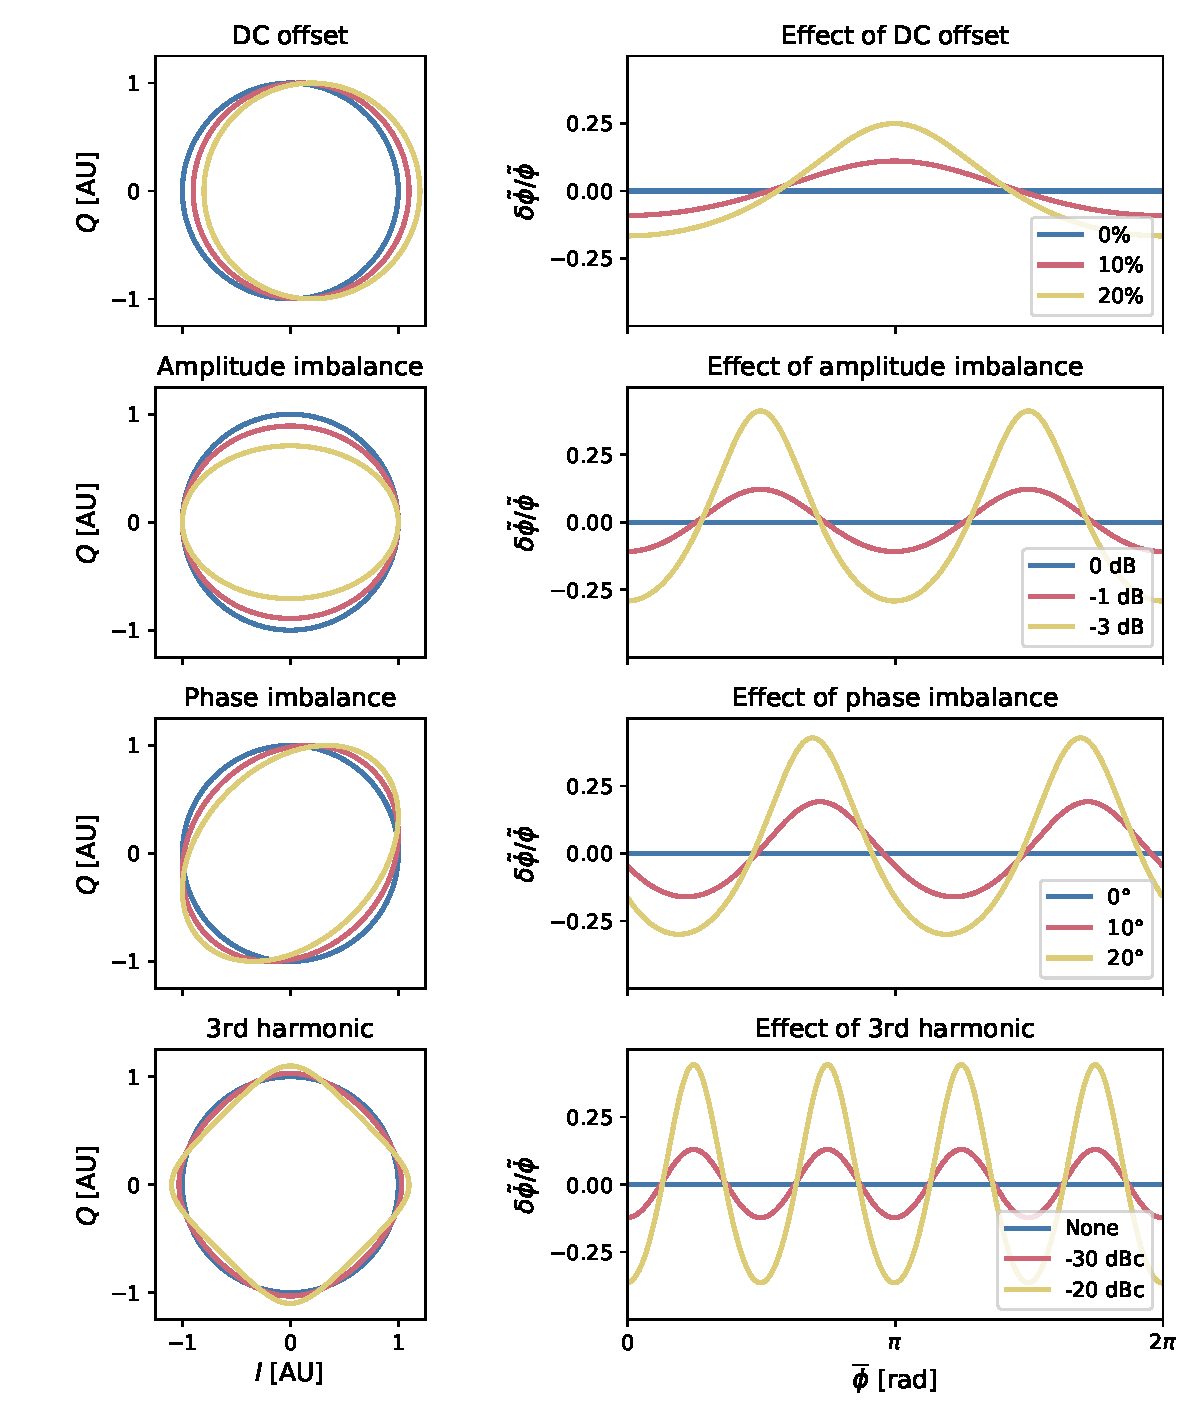
\includegraphics[width = \textwidth]{%
    Chapters/DesignConsiderations/figs/demodulator_imperfections.pdf}
  \caption[Effects of demodulator imperfections]{%
    Demodulator imperfections produce errors in the measured phase.
    The left column displays the Lissajous curves
    that result from plotting
    the quadrature $Q$ vs.\ in-phase $I$ signals, while
    the right column plots the relative error
    $\delta\tilde{\phi} / \tilde{\phi}$
    in the measured fluctuating phase
    as a function of the equilibrium phase $\bar{\phi}$.
    Each row examines a different demodulator imperfection.
  }
  \label{fig:DesignConsiderations:effects_of_demodulator_imperfections}
\end{figure}


\section{Quantization noise}
\label{sec:DesignConsiderations:quantization}
Efficient conversion of an analog signal to a digital record requires
quantization of the signal magnitude and
temporal sampling of these quantized magnitudes~\cite{bennett_bstj48}.
This analog-to-digital conversion
is performed by an instrument known as a digitizer.
If a digitizer has bit depth $N_b$ and
an input-voltage dynamic range $V_{\text{dyn}}$,
then its quantum of voltage $\Delta V$ is
\begin{equation}
  \Delta V
  =
  \frac{V_{\text{dyn}}}{2^{N_b} - 1}
  \approx
  \frac{V_{\text{dyn}}}{2^{N_b}},
  \label{eq:DesignConsiderations:digitizer_voltage_quantum}
\end{equation}
where the approximation is well-satisfied
for typical digitizer bit depths.
At each sampling time,
the analog signal's magnitude is approximated
by the closest quantized value, whose
separation from the true, analog value
will be less than or equal to $\Delta V / 2$.

In general, then, the quantized signal
will differ from the analog signal.
This error $\epsilon$ is known as quantization noise.
The mean square error (i.e.\ variance) attributable to quantization is simply
\begin{equation}
  \overline{\epsilon^2} = \frac{(\Delta V)^2}{12},
  \label{eq:DesignConsiderations:quantization_noise_variance}
\end{equation}
where $\Delta V$ is the digitizer's quantum of voltage,
as given by (\ref{eq:DesignConsiderations:digitizer_voltage_quantum})
\cite{bennett_bstj48}
\cite[Sec.~10.2.4]{bendat_and_piersol}.
For a uniformly sampled record with sampling rate $f_s$,
sufficiently fine quantization $\Delta V$
ensures that the quantization noise is \emph{white}
\cite[Th.~1]{bennett_bstj48}
\cite[Ch.~20]{widrow_and_kollar};
that is, the one-sided autospectral density of the quantization noise is
\begin{align}
  G_{\epsilon,\epsilon}(f)
  =
  \frac{\overline{\epsilon^2}}{f_s / 2}
  =
  \frac{(\Delta V)^2}{6 f_s},
  \qquad
  0 \leq f \leq \frac{f_s}{2}.
  \label{eq:DesignConsiderations:quantization_noise_autospectral_density}
\end{align}
In practice, however, aperture error, jitter, and nonlinearities
may reduce the effective bit depth by one or two bits
\cite[Sec.~10.2.4]{bendat_and_piersol},
increasing the realized quantization noise
relative to that expected from
(\ref{eq:DesignConsiderations:quantization_noise_variance}) and
(\ref{eq:DesignConsiderations:quantization_noise_autospectral_density}).

Quantization noise can be significant
when attempting to measure absolute phase fluctuations
with a heterodyne interferometer.
Recall from the discussion of heterodyne interferometric detection in
Section~\ref{sec:InterferometricMethods:interferometry:heterodyne}
that measurement of the \emph{absolute} phase
requires capturing the full dynamics
of the large, slowly varying equilibrium phase $\bar{\phi}$
in addition to measuring the fluctuating phase $\tilde{\phi}$.
Because $\tilde{\phi} \ll \bar{\phi}$ in typical situations,
the fluctuations only occupy a small portion
of the digitizer's dynamic range; that is,
fluctuations effectively see a bit depth that
is substantially smaller than the digitizer's nominal bit depth.
Thus, to minimize the effect of quantization noise,
it is absolutely imperative
to utilize the full dynamic range of the digitizer.


\bibliographystyle{plainurl}
\bibliography{references}
